\documentclass{article}

% Package for setting page margins
\usepackage[top=1cm, bottom=1cm, left=2cm, right=2cm]{geometry}
\newif\ifincludeimages
\includeimagestrue % Include images by default

% Package for better font handling
\usepackage[T1]{fontenc}
\usepackage[utf8]{inputenc}
\usepackage{lmodern}
\usepackage{qrcode}
\usepackage{xcolor}
\usepackage{titlesec}
\usepackage{enumitem} 
\usepackage{graphicx}
\usepackage{parallel} % for parallel environment

\titleformat{\section}{\large\bfseries}{\thesection}{1em}{}

% Package for customizing itemized lists
\usepackage{enumitem}
\setlist[itemize]{leftmargin=*}
 \usepackage[colorlinks=true, citecolor={red!70!black}, linkcolor={red!40!black}, urlcolor={blue!40!black}, pdfborder={0 0 0}]{hyperref}
 
% Package for including images
\usepackage{graphicx}
\usepackage{multicol}

\begin{document}


\pagestyle{empty} % Remove page numbers

% Header section with image
\begin{center}
    \begin{minipage}[t]{0.2\textwidth}
        \vspace{0pt}
        
\includegraphics[width=3cm]{img.png}
    \end{minipage}
    \hspace{1cm}
    \begin{minipage}[t]{0.7\textwidth}
        \vspace{0pt}
        \textbf{CURRICULUM VITAE}\\\\
        \textbf{Name:} Lic. Javier Alejandro Oramas López\\
        \\
        \textbf{Phone:} +34 637 85 47 65 \\
        \textbf{Email:} javiale2000@gmail.com \\
        \textbf{Date of Birth:}  02/25/2000\\
        \textbf{github:} \href{https://github.com/JavierOramas}{JavierOramas} \\
        \textbf{linkedin:} \href{https://www.linkedin.com/in/javier-alejandro-oramas-l%C3%B3pez-7ab47b160/}{javier-alejandro-oramas} \\
    \end{minipage}
\end{center}

% Experience section
\section*{Experience}
    \textbf{Tech Consultant and DevOps} \hfill since \textbf{ 2019 }\\ 
    WamasolTech, 
    \href{https://wamasol.com}{Wamasol}\\
    \vspace{0.1cm}\\
    \textbf{Trained Professor (Computer Networks)} \hfill \textbf{ 2024}\\ 
    \href{https://matcom.uh.cu}{MATCOM, UH}\\
    \vspace{0.1cm}\\
    \textbf{Backend Developer} \hfill since \textbf{10/2023}\\ 
    Fonoma LLC, (remote)
    \href{https://fonoma.com}{Fonoma}\\
    Mostly working in django, fastapi, nodejs, unit test and DevOps\\
    \vspace{0.1cm}\\
    \textbf{Developer} \hfill \textbf{2021-2025}\\ 
    American Behavioral Solutions, Arizona (remote)
    \href{https://americanbehavioralsolutions.com}{ABS}
    Development and deployment of a Management system to control Supervisions

% Education section
\section*{Education}
\textbf{Research Intern (AI)} \hfill \textbf{2023-2024}\\
\href{https://matcom.in/}{MATCOM}, \href{https://uh.cu}{Universidad de La Habana}, Cuba\\
\href{https://www.colmex.mx/}{El Colegio de M\'exico}, CDMX, M\'exico\\
\vspace{0.1cm}\\
\textbf{Bachelors Degree in Computer Science} \hfill \textbf{2018-2024}\\
\href{https://matcom.in/}{MATCOM}, \href{https://uh.cu}{Havana University}, Cuba\\
\vspace{0.1cm}\\
\textbf{\hyperref[sec:bachelor]{Science Bachelor}} \hfill \textbf{2018}\\
Vocational Institute of Exact Sciences  Ernesto Guevara, Cuba

% Skills section
\section*{Skills}
\begin{multicols}{3}

\textbf{Programming Languages}
\begin{itemize}
    \item 
\includegraphics[height=10pt]{images/icons/python.png} Python
    \item 
\includegraphics[height=10pt]{images/icons/c.png} C
    \item 
\includegraphics[height=10pt]{images/icons/cpp.png} C++
    \item 
\includegraphics[height=10pt]{images/icons/csharp.png} C\#
    \item 
\includegraphics[height=10pt]{images/icons/mysql-original.png} SQL
    \item 
\includegraphics[height=10pt]{images/icons/rust-plain.png} Rust
    \item 
\includegraphics[height=10pt]{images/icons/go-original-wordmark.png} Go
    \item 
\includegraphics[height=10pt]{images/icons/dart.png} Dart
    \item 
\includegraphics[height=10pt]{images/icons/javascript-original} Javascript
    \item 
\includegraphics[height=10pt]{images/icons/latex-original.png} LaTeX
    \item 
\includegraphics[height=10pt]{images/icons/bash-original.png} Bash
\end{itemize}

\textbf{Other Technologies}
\begin{itemize}
    \item 
\includegraphics[height=10pt]{images/icons/sklearn.png} SKLearn
    \item 
\includegraphics[height=10pt]{images/icons/tensorflow-original.png} Tensorflow
    \item 
\includegraphics[height=10pt]{images/icons/pytorch-original.png} Pytorch
    \item 
\includegraphics[height=10pt]{images/icons/pandas-original.png} Pandas
    \item 
\includegraphics[height=10pt]{images/icons/numpy-original.png} Numpy
    \item 
\includegraphics[height=10pt]{images/icons/docker.png} Docker
    \item 
\includegraphics[height=10pt]{images/icons/git-original.png} Git
    \item 
\includegraphics[height=10pt]{images/icons/github-original.png} Github
    \item 
\includegraphics[height=10pt]{images/icons/pytest-original.png} Pytest
    \item 
\includegraphics[height=10pt]{images/icons/selenium-original.png} Selenium
    \item 
\includegraphics[height=10pt]{images/icons/fastapi-original.png} Fastapi
    \item 
\includegraphics[height=10pt]{images/icons/bootstrap.png} Bootstrap
    \item 
\includegraphics[height=10pt]{images/icons/flutter-original.png} Flutter
    \item 
\includegraphics[height=10pt]{images/icons/dotnetcore.png} Dotnetcore
    \item 
\includegraphics[height=10pt]{images/icons/typer.png} Typer
    \item 
\includegraphics[height=10pt]{images/icons/bs.png} Beautiful soup
    \item 
\includegraphics[height=10pt]{images/icons/mongodb-original.png} MongoDB
    \item 
\includegraphics[height=10pt]{images/icons/sqlalchemy-original.png} SQLAlchemy
\end{itemize}

\end{multicols}


% Personal Projects section
\IfFileExists{build/projects.tex}{
    \section*{Personal Projects}
    \input{build/projects.tex}
}{}

\IfFileExists{build/Events.tex}{

    \section*{Events}
    \input{build/events.tex}
}{}

\IfFileExists{build/awards.tex}{
\section*{Awards and Distinctions}

\begin{minipage}{0.8\textwidth}
    \parbox{0.8\linewidth}{\textbf{Relevant thesis for the AI tribunal}} \hfill \textbf{12/2022}\\
    \href{https://github.com/JavierOramas/thesis_experiments}{Thesis}
    \href{https://github.com/JavierOramas/thesis}{Thesis Document}
    \\
\begin{minipage}{0.8\textwidth}
    \parbox{0.8\linewidth}{\textbf{Best Prediction in the world at FIFA World Cup}} \hfill \textbf{12/2022}\\
    \href{https://www.postdata.club/suplementos/mundial-qatar/pronosticando-qatar.html}{postdata.club}
    \\
\end{minipage} \hfill \qrcode[height=0.6in]{https://www.postdata.club/suplementos/mundial-qatar/pronosticando-qatar.html}\\
\begin{minipage}{0.8\textwidth}
    \parbox{0.8\linewidth}{\textbf{Best preditction int the world (for cuban delegation results) at Lima 2019 Panamerican Games, using Machine Learning}} \hfill \textbf{07/2019}\\
    \href{http://www.postdata.club/issues/201907/el-medallero-de-lima-2019-que-se-puede-esperar.html}{postdata.club}
    \\
\end{minipage} \hfill \qrcode[height=0.6in]{https://github.com/JavierOramas/PanamericanPredictor}\\
\begin{minipage}{0.8\textwidth}
    \parbox{0.8\linewidth}{\textbf{3rd place MATCOM Game Festival 2019, Videogame "El Origen"}} \hfill \textbf{02/2019}\\
    \\
\end{minipage}\\
\begin{minipage}{0.8\textwidth}
    \parbox{0.8\linewidth}{\textbf{13th place in the Caribbean, ACM-ICPC 2018 national Contest,  UH-KEJ (Participating as a team representing Havana University)}} \hfill \textbf{10/2018}\\
    \href{https://icpc.global/regionals/finder/cnc-2018/standings}{standings}
    \\
\end{minipage} \hfill \qrcode[height=0.6in]{https://icpc.global/regionals/finder/cnc-2018/standings}\\
\begin{minipage}{0.8\textwidth}
    \parbox{0.8\linewidth}{\textbf{7th place ACM-ICPC 2018 Local Contest, UH-KEJ (Participating as a team representing Havana University)}} \hfill \textbf{07/2018}\\
    \href{https://matcomgrader.com/post/5179/resultados-del-concurso-local-caribeno-2018}{standings}
    \\
\end{minipage} \hfill \qrcode[height=0.6in]{https://matcomgrader.com/post/5179/resultados-del-concurso-local-caribeno-2018}\\
\begin{minipage}{0.8\textwidth}
    \parbox{0.8\linewidth}{\textbf{Granted directly, by resolution of the Ministry of Education the career: Computer Science at Universidad de La Habana, According to the achievents in  the ACM-ICPC 2017 Caribbean Finals.}} \hfill \textbf{06/2018}\\
    \\
\end{minipage} \\
\begin{minipage}{0.8\textwidth}
    \parbox{0.8\linewidth}{\textbf{26th place in the Caribbean y 200th in LATAM, ACM-ICPC Caribbean Finals, Team3C-1 (Participating as  Invited Team from pre-universitary schools)}} \hfill \textbf{11/2017}\\
    \href{https://matcomgrader.com/media/posts/5167/ranking/caribbean.png}{Region Standing}
    \href{https://matcomgrader.com/media/posts/5167/ranking/general.png}{Continent Standing}
    \\
\end{minipage} \hfill \qrcode[height=0.6in]{https://matcomgrader.com/media/posts/5167/ranking/caribbean.png}\\
\begin{minipage}{0.8\textwidth}
    \parbox{0.8\linewidth}{\textbf{5th Place in Cuban Finals of ACM-ICPC, Team3C-1}} \hfill \textbf{10/2017}\\
    \\
\end{minipage}\\
\begin{minipage}{0.8\textwidth}
    \parbox{0.8\linewidth}{\textbf{Third Place in "UCLV CUP" proggramming contest at Universidad Central Marta Abreu de Las Villas}} \hfill \textbf{06/2017}\\
    \\
\end{minipage}\\
\begin{minipage}{0.8\textwidth}
    \parbox{0.8\linewidth}{\textbf{1st place Cuban National Programming Contest}} \hfill \textbf{01/2017}\\
    \\
\end{minipage}\\
\begin{minipage}{0.8\textwidth}
    \parbox{0.8\linewidth}{\textbf{4th place Lenin Cup}} \hfill \textbf{01/2017}\\
    \\
\end{minipage}\\
\begin{minipage}{0.8\textwidth}
    \parbox{0.8\linewidth}{\textbf{1st place at UCLV site ACM-ICPC National Finals 2015-2016 }} \hfill \textbf{10/2015}\\
    \\
\end{minipage} \\
\begin{minipage}{0.8\textwidth}
    \parbox{0.8\linewidth}{\textbf{3rd  place at UCLV site ACM-ICPC Local Finals 2015-2016 (Participating as  Invited Team from pre-universitary schools)}} \hfill \textbf{09/2015}\\
    \\
\end{minipage}\\

\begin{minipage}{0.8\textwidth}
    \parbox{0.8\linewidth}{\textbf{Research Group in Artifitial Intelligence at Facultad de Matemática y Computación de la Universidad de La Habana (Computer Science and Mathematics Faculty, Havana University)
    }} \hfill \textbf{Since 2019}\\
    \\
\end{minipage}\\
\begin{minipage}{0.8\textwidth}
    \parbox{0.8\linewidth}{\textbf{Cuban National pre-selection to the Intenational Olimpiad in Informatics
    }} \hfill \textbf{04/2016-07/2016}\\
    \\
\end{minipage}\\
\begin{minipage}{0.8\textwidth}
    \parbox{0.8\linewidth}{\textbf{Provincial Contest Center, Villa Clara, Cuba
    }} \hfill \textbf{04/2016-07/2016}\\
    \\
\end{minipage}\\

\newpage}{}

\IfFileExists{build/attachments.tex}{\section*{Attachments}
% \begin{minipage}{0.8\textwidth}
\begin{figure}[h]
    
\includegraphics[width=\textwidth]{images/bachelor.png}
    \caption{Science Bachelor certificate}
    \label{sec:bachelor}
\end{figure}

\begin{figure}[h]
    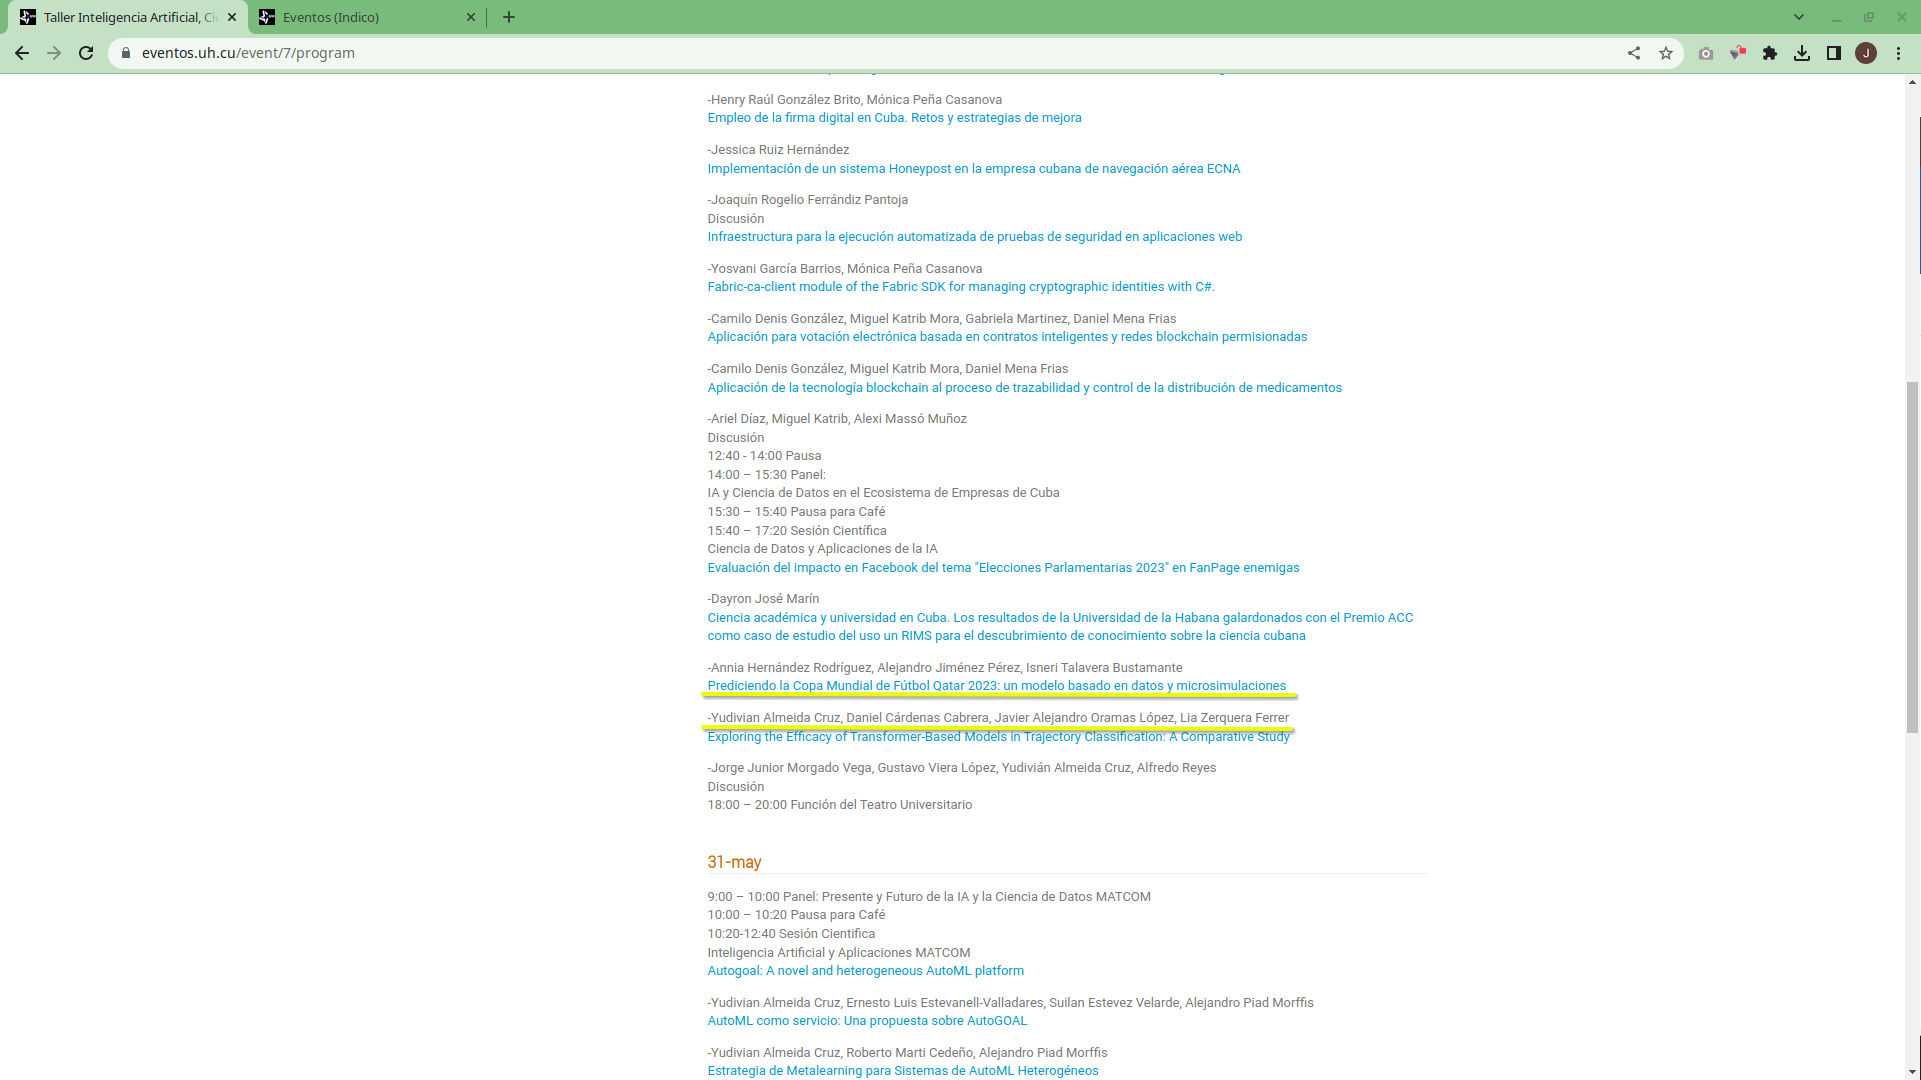
\includegraphics[width=\textwidth]{images/ai_workshop.png}
    \caption{\href{https://eventos.uh.cu/event/7/program}{Havana University events webpage}, screenshot 06/01/2023}
    \label{sec:workshop}
\end{figure}

\begin{figure}[h]
    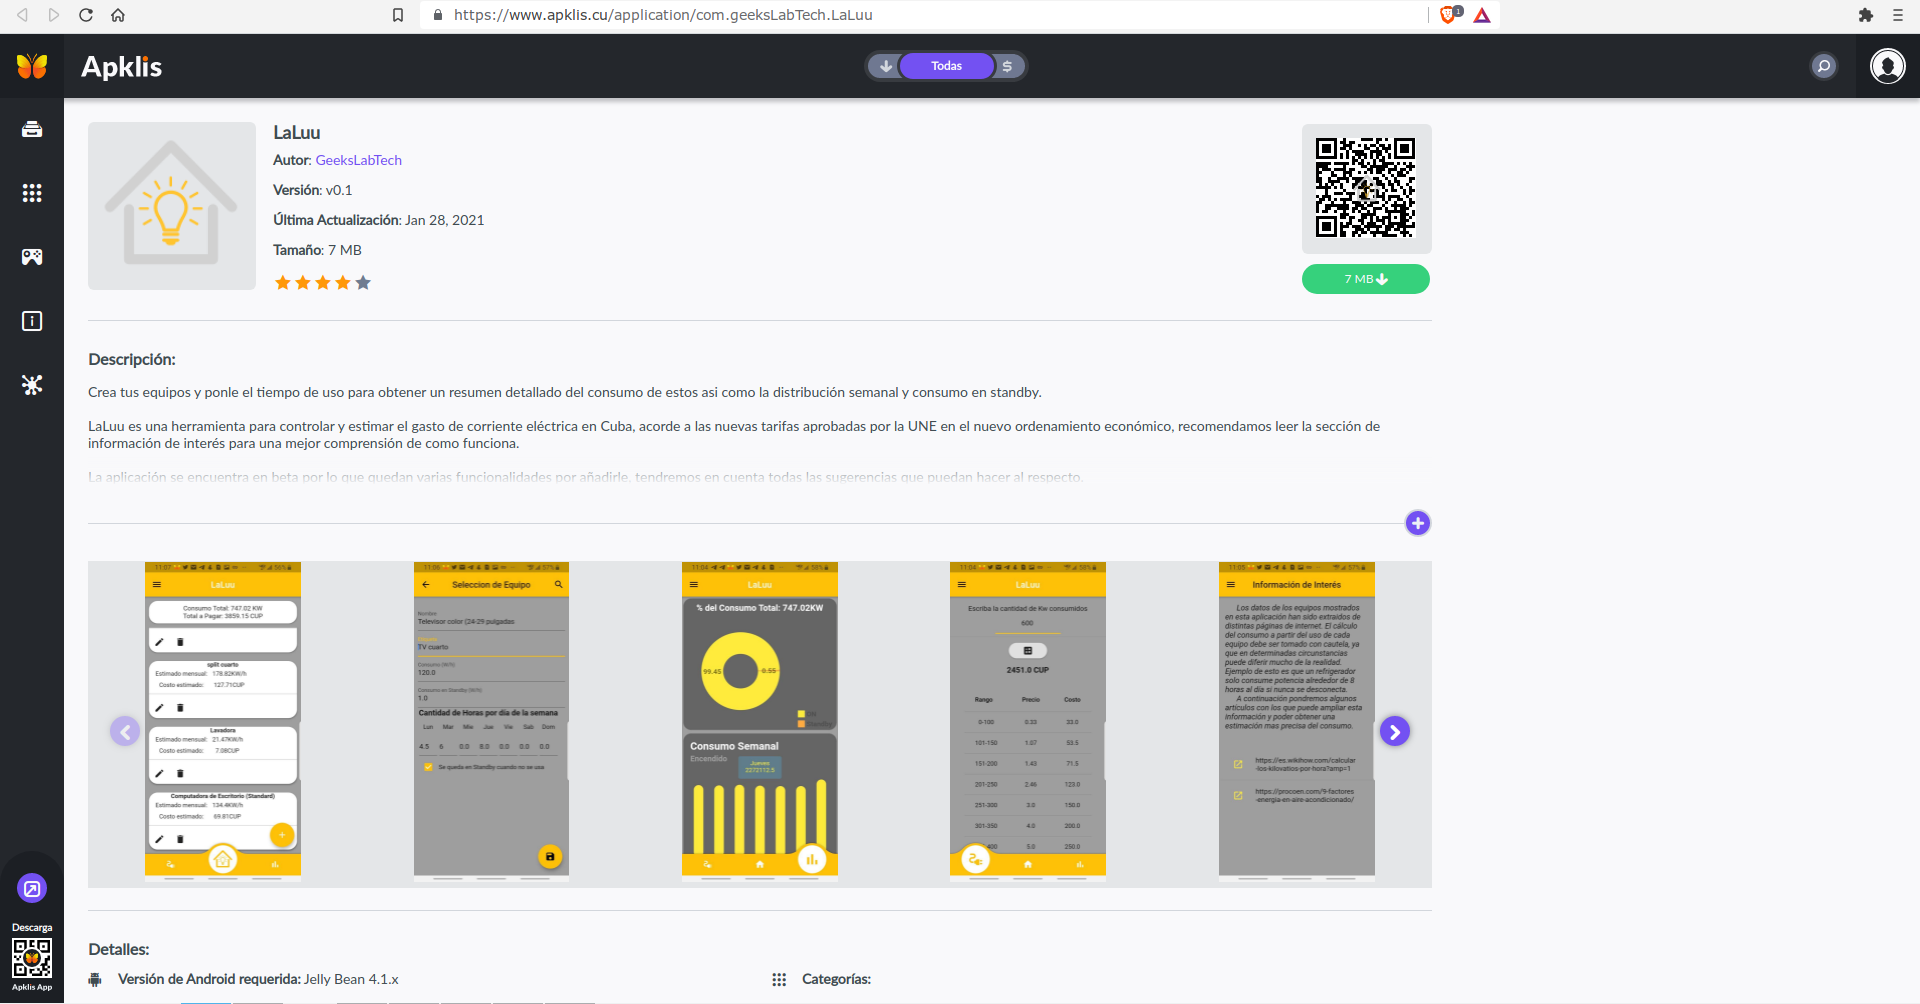
\includegraphics[width=\textwidth]{images/laluu.png}
    \caption{LaLuu app for estimation of Energy consumption. Available in \href{https://www.apklis.cu/application/com.geeksLabTech.LaLuu}{Apklis}, Cuban android app store, screenshot 01/25/2022}
    \label{sec:laluu}
\end{figure}

\begin{figure}[h]
    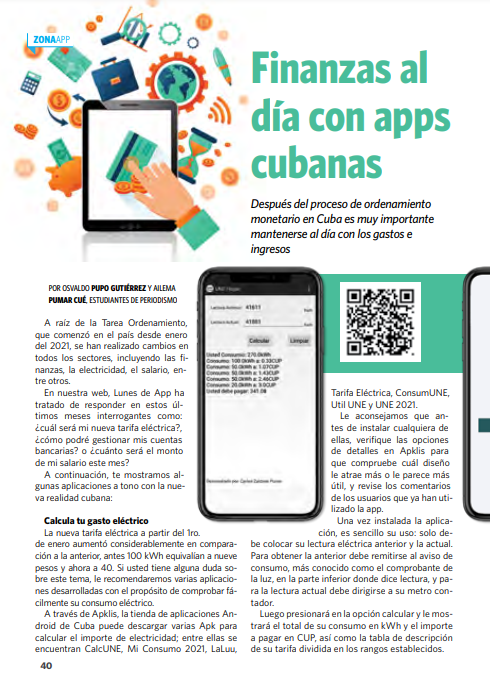
\includegraphics[width=\textwidth]{images/laluu_jt.png}
    \caption{Pupo, Gutiérrez O. y Pumar, Cué A. (may-jun 2021). \href{http://www.juventudtecnica.cu/sites/default/files/jt_420.pdf}{Finanzas al día con apps cubanas}. Juventud Técnica 420 (40-41), ISSN: 0449-4555, screenshot 01/25/2022}
    \label{sec:laluu_press}
\end{figure}

\begin{figure}[h]
    
\includegraphics[width=\textwidth]{images/laluu_art.png}
    \caption{Red Artemisa (february 2nd 2021).\href{https://www.artemisa.gob.cu/es/actualidad/noticias/9806-llego-febrero-calcula-tu-gasto-electrico-con-esta-apps}{Llegó febrero: calcula tu gasto eléctrico con esta apps.}, screenshot 01/25/2022}
\end{figure}

\begin{figure}[h]
    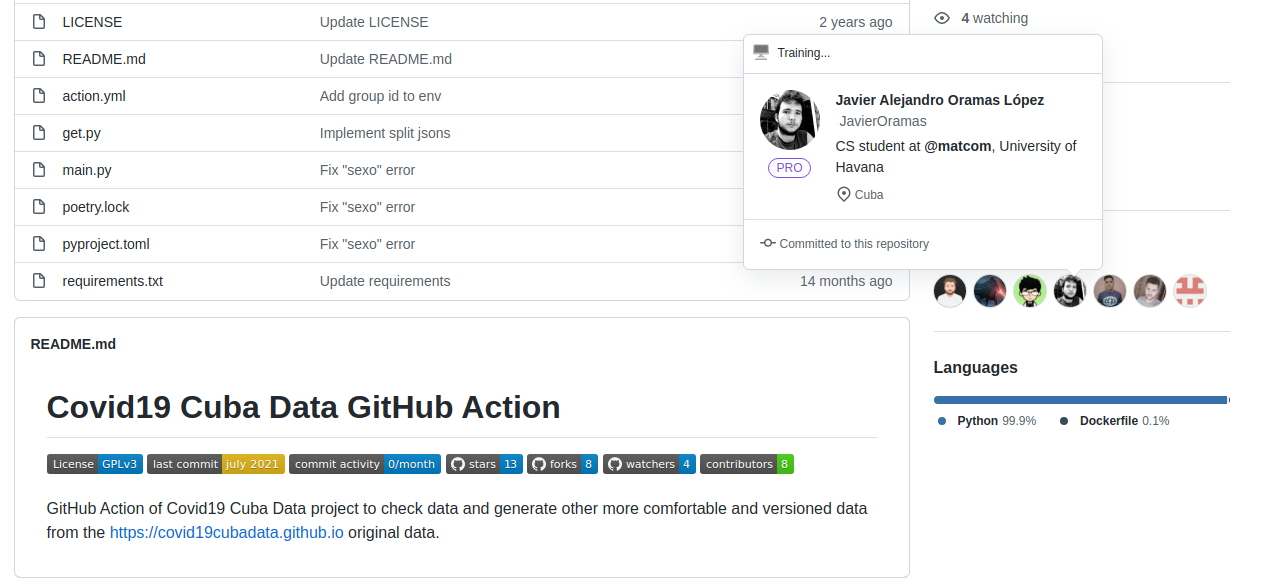
\includegraphics[width=\textwidth]{images/covid_19.png}
    \caption{\href{https://github.com/covid19cuba/covid19cuba-action}{Covid19CubaData app COVID-19 data analisys in Cuba}, screenshot 01/25/2022}
    \label{sec:covid}
\end{figure}

\begin{figure}[h]
    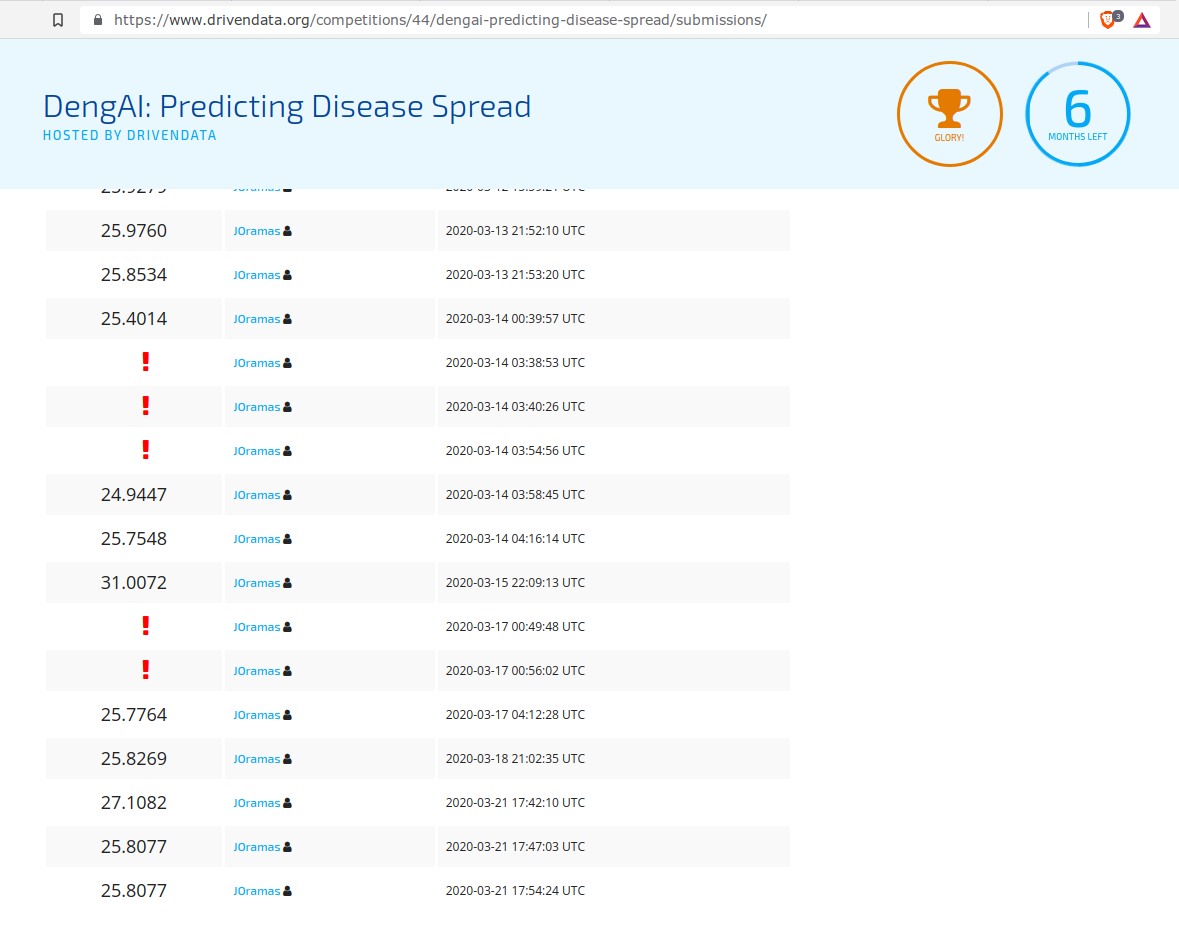
\includegraphics[width=\textwidth]{images/dengue.png}
    \caption{Competition Predicting Dengue Cases based on metheorological variables, using Machine Learning and Deep Learning. \href{https://www.drivendata.org/competitions/44/dengai-predicting-disease-spread}{DrivenData}, screenshot 01/25/2022}
    \label{sec:dengue}
\end{figure}

\begin{figure}[h]
    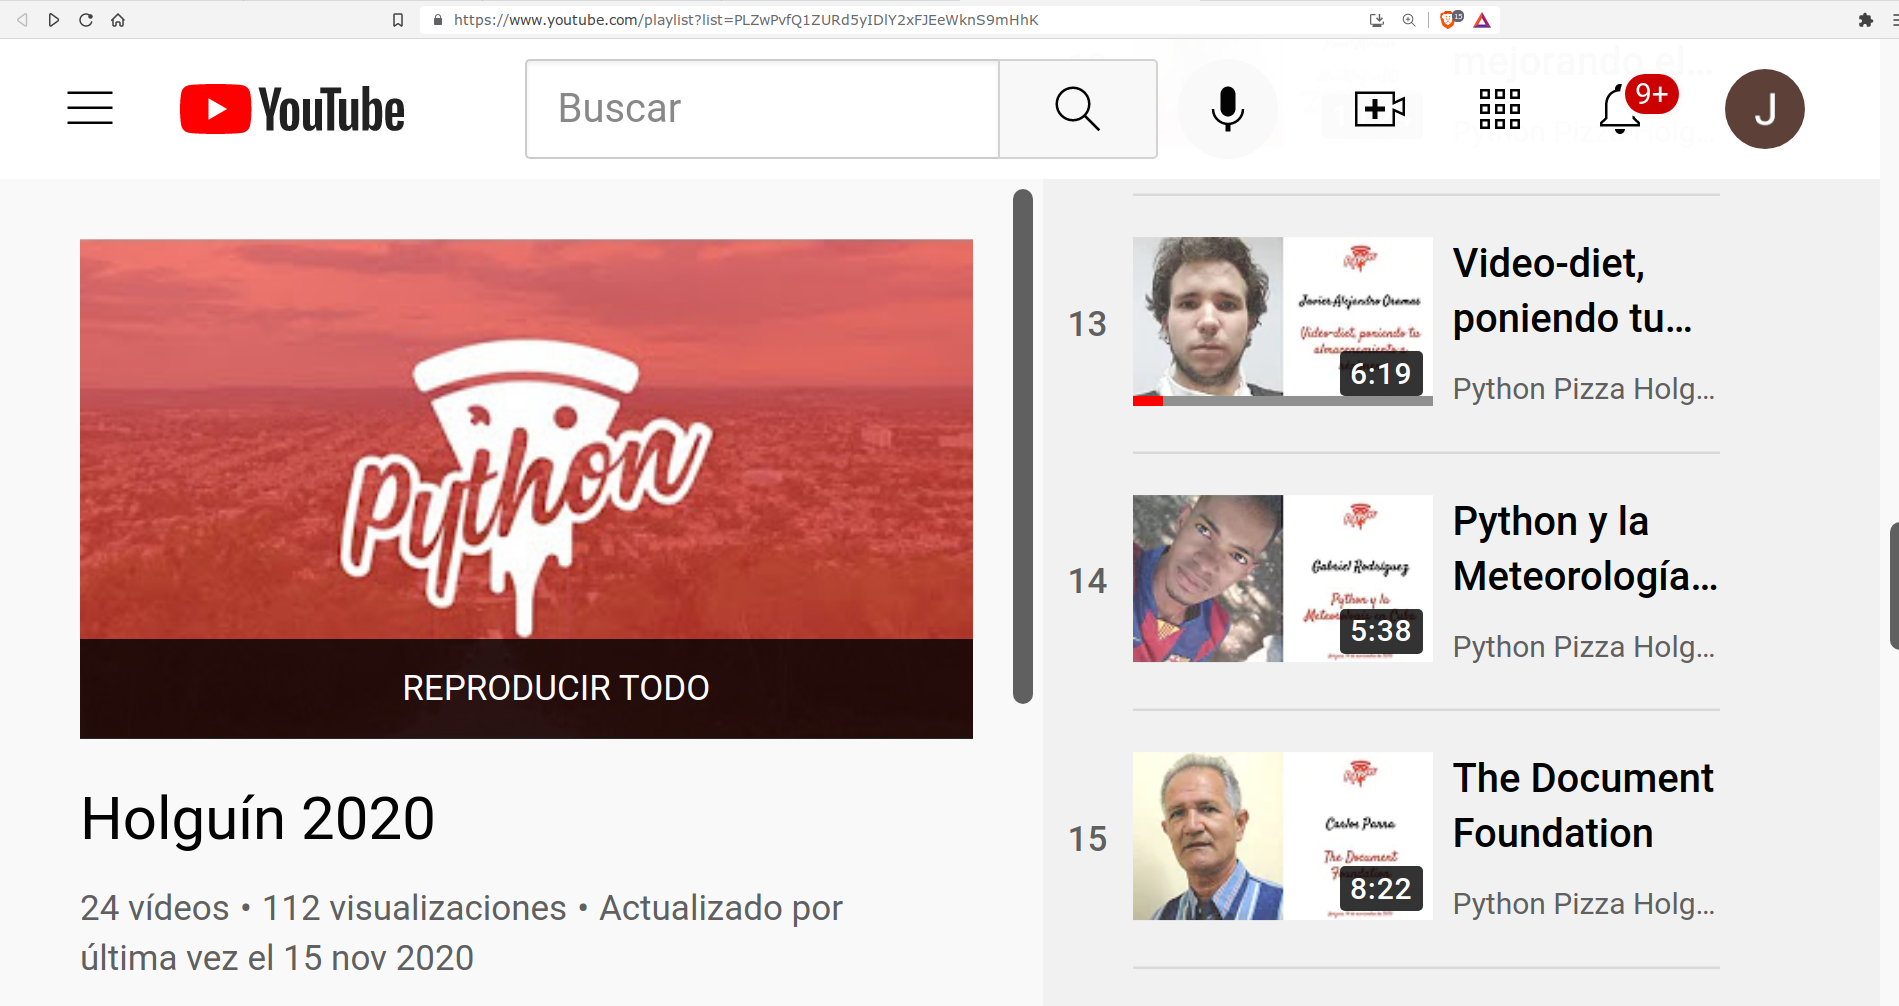
\includegraphics[width=\textwidth]{images/pythonpizza.png}
    \caption{Oramas, J. \href{https://holguin.python.pizza/?ref=python.pizza}{[Python Pizza Holguín]}. (nov 15th 2020). Video-Diet: poniendo a dieta tu almacenamiento \href{https://youtu.be/c--NOwM5W-0}{[Video]}.screenshot 01/25/2022}
    \label{sec:pythonpizza}
\end{figure}

\begin{figure}[h]
    \centering
    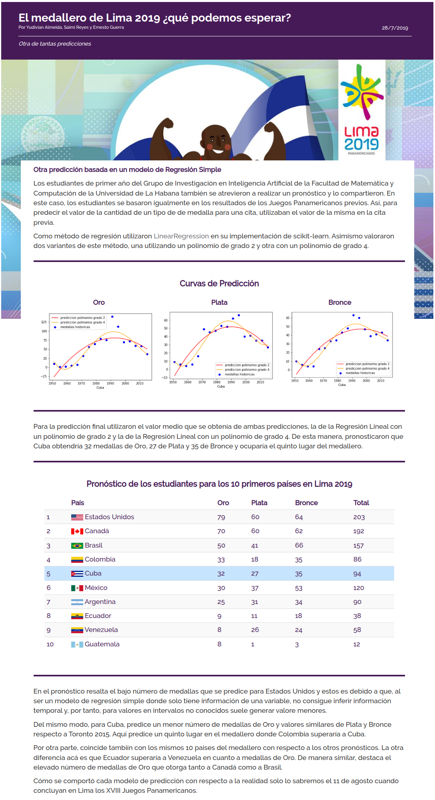
\includegraphics[height=0.8\textheight]{images/panamerican.png}
    \caption{\href{http://www.postdata.club/issues/201907/el-medallero-de-lima-2019-que-se-puede-esperar.html}{Almeida, Y. , Reyes, S. y Guerra, E. (jul 28th 2019). El medallero de Lima 2019 ¿qué podemos esperar? PostData.club Periodismo de Datos.}, screenshot 01/25/2022}
    \label{sec:panamerican}
\end{figure}

\begin{figure}[h]
    \centering
    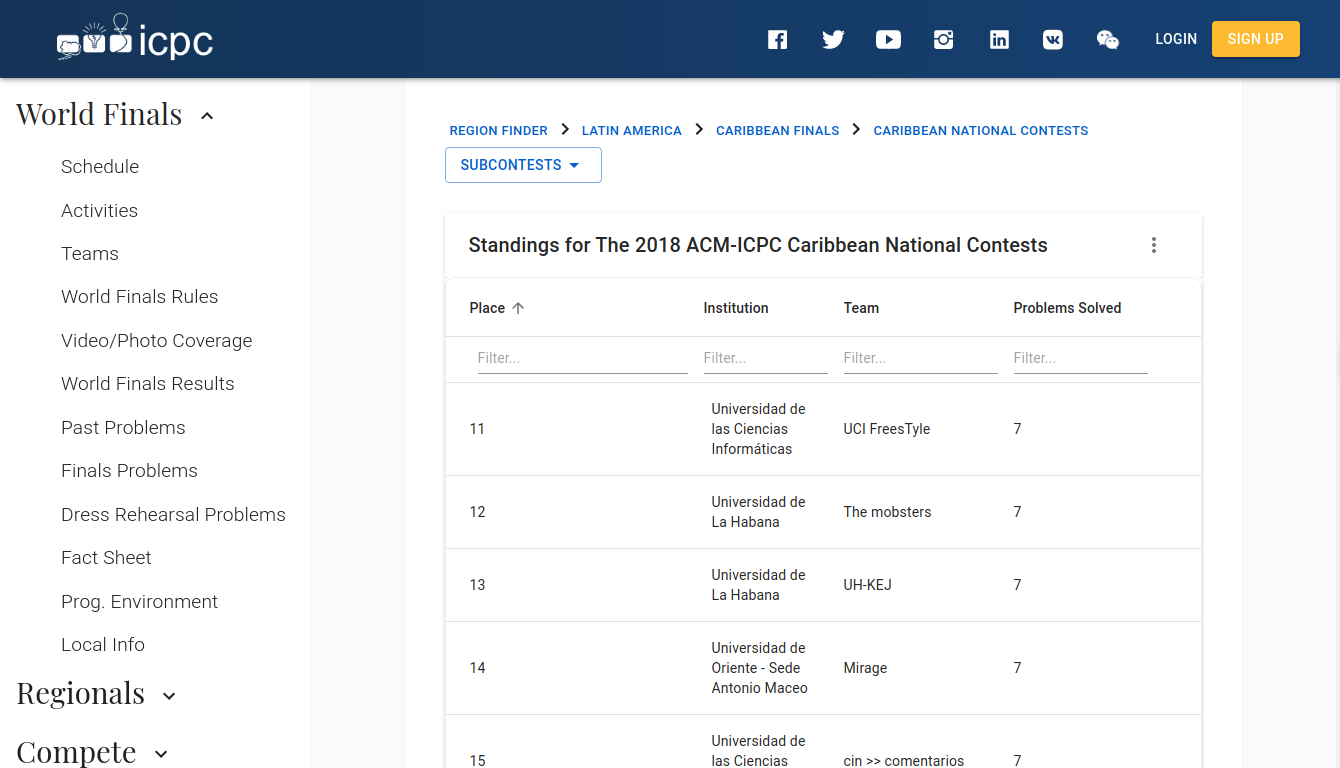
\includegraphics[width=\textwidth]{images/icpckej.png}
    \caption{ \href{https://icpc.global/regionals/finder/cnc-2018/standings}{International Collegiate Programming Contest (oct 2018). Standings for The 2018 ACM-ICPC Caribbean National Contests}. screenshot 01/25/2022}
    \label{sec:icpc_kej}
\end{figure}

\begin{figure}[h]
    \centering
    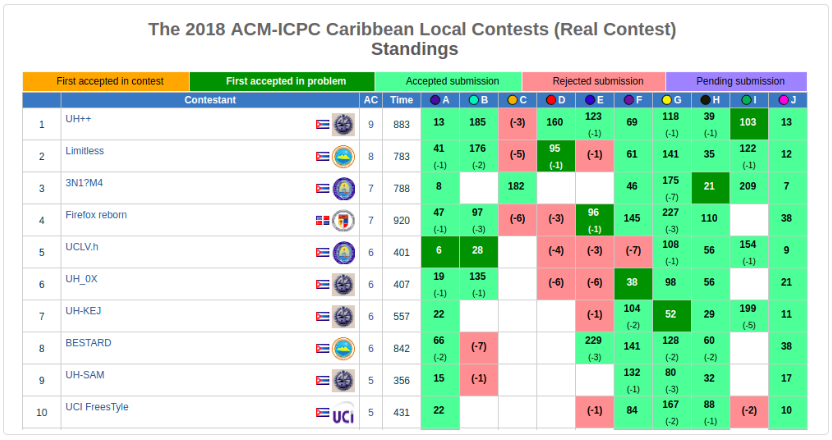
\includegraphics[width=\textwidth]{images/icpckej_standing.png}
    \caption{\href{https://matcomgrader.com/post/5179/resultados-del-concurso-local-caribeno-2018}{Matcom Online Grader (sept 2018). Resultados del Concurso Local Caribeño 2018. Facultad de Matemática y Ciencia de la Computación, Universidad de La Habana.}, screenshot 01/25/2022}
    % \label{sec:}
\end{figure}

\begin{figure}[h]
    \centering
    
\includegraphics[width=\textwidth]{images/letter.png}
    \caption{General Director invitation letter, Caribbean Finals ACM - ICPC 2017, screenshot 01/25/2022}
    \label{sec:letter}
\end{figure}

\begin{figure}[h]
    \centering
    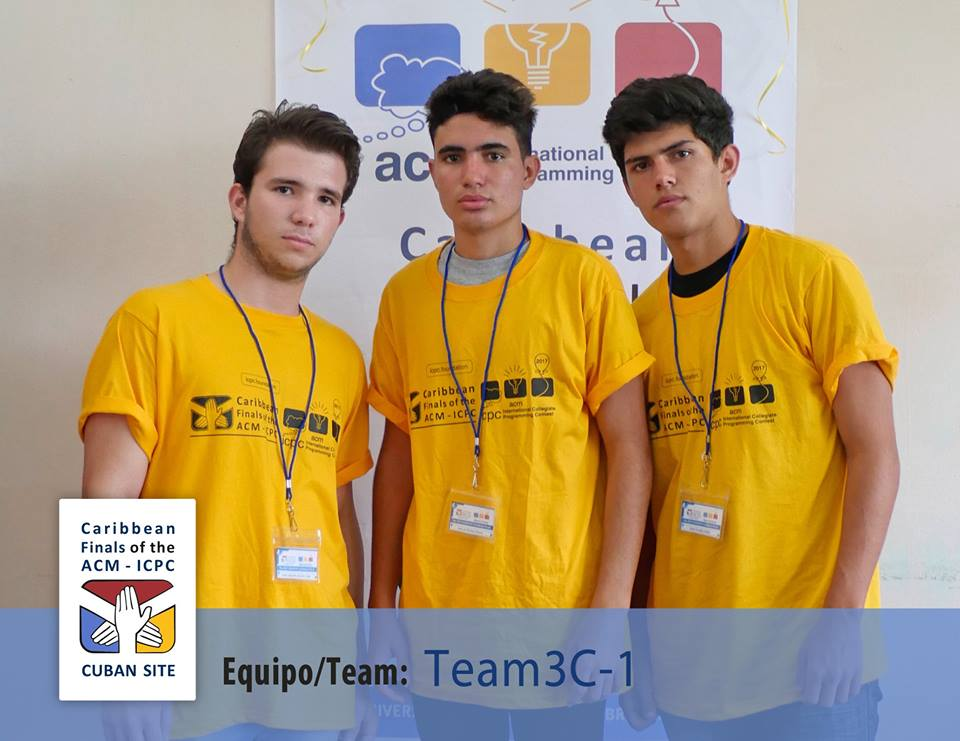
\includegraphics[width=\textwidth]{images/team3c.jpg}
    \caption{\href{https://matcomgrader.com/post/5167/the-2017-acm-icpc-caribbean-finals}{Matcom Online Grader (oct 2017). The 2017 ACM-ICPC Caribbean Finals. Facultad de Matem?tica y Ciencia de la Computaci?n, Universidad de La Habana} screenshot 01/25/2022}
    \label{sec:3c}
\end{figure}
\begin{figure}[h]
    \centering
    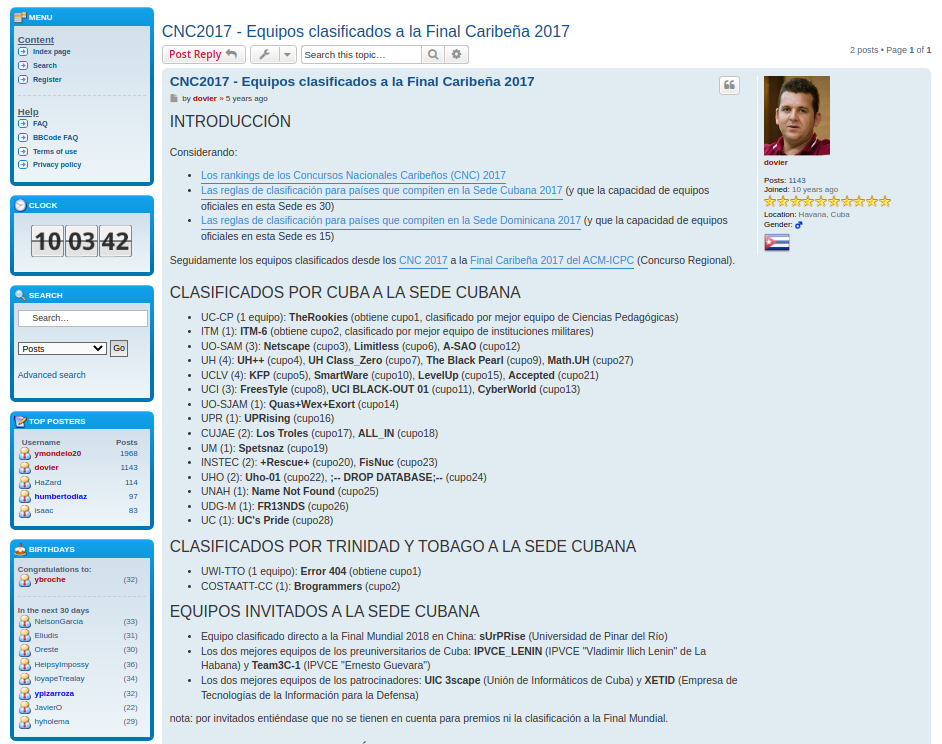
\includegraphics[width=\textwidth]{images/icpc_classified.png}
    \caption{\href{ https://coj-forum.uci.cu/viewtopic.php?t=3315}{Caribbean Online Judge (nov 2017). Final Caribe?a del ACM - ICPC 2017.}, screenshot 01/25/2022}
    \label{sec:icpc}
\end{figure}

\begin{figure}[h]
    \centering
    
\includegraphics[width=\textwidth]{images/2017final.png}
    \caption{Participation Certificate, ACM-ICPC 2017 Cuban Finals, screenshot 01/25/2022}
    \label{sec:2017final}
\end{figure}


\begin{figure}[h]
    \centering
    
\includegraphics[width=\textwidth]{images/uclv_cup.png}
    \caption{Participation Certificate, IV Programming Cup, Universidad Central de Las Villas, screenshot 01/25/2022}
    \label{sec:uclv_cup}
\end{figure}


\begin{figure}[h]
    \centering
    
\includegraphics[width=\textwidth]{images/nac_contest.png}
    \caption{Certificate for Relevant Results obtained in the National Informatics Competition, Mach 2017, screenshot 01/25/2022}
    \label{sec:nac_contest}
\end{figure}


\begin{figure}[h]
    \centering
    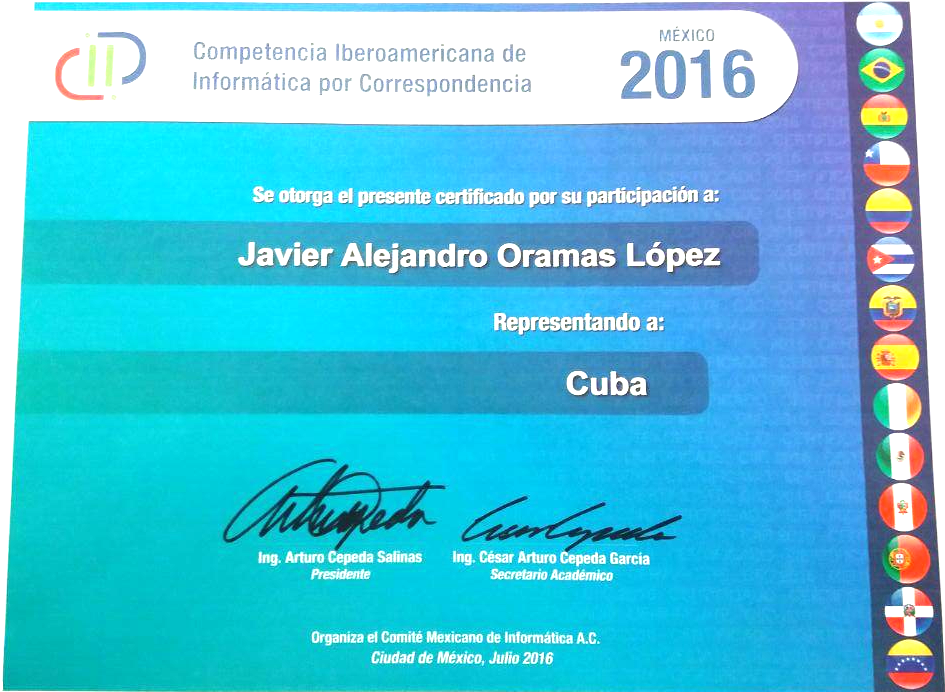
\includegraphics[width=\textwidth]{images/ibero.png}
    \caption{Certificate of Participation, Iberoamerican Computer Correspondence Competition, México 2016, screenshot 01/25/2022}
    \label{sec:ibero}
\end{figure}


\begin{figure}[h]
    \centering
    
\includegraphics[width=\textwidth]{images/preseleccion.png}
    \caption{Certificate from the Ministry of Education of Cuba for having integrated the National Preselection to the International Olympiads of Informatics. 2016, screenshot 01/25/2022}
    \label{sec:preseleccion}
\end{figure}


\begin{figure}[h]
    \centering
    
\includegraphics[width=\textwidth]{images/tinajon.png}
    \caption{Certificate for Third place obtained in the Regional Cup of Computer Science Competition, Camag\"uey December 2015, screenshot 01/25/2022}
    \label{sec:tinajon}
\end{figure}


\begin{figure}[h]
    \centering
    \includegraphics[width=\textwidth]{images/2016nacional.png}
    \caption{Certificate of participation in the National Competition of the ACM-ICPC, Universidad Central de Las Villas, October 2015, screenshot 01/25/2022}
    \label{sec:nacional2016}
\end{figure}


\begin{figure}[h]
    \centering
    \includegraphics[width=\textwidth]{images/2016local.png}
    \caption{Certificate of participation in the Local Competition of the ACM-ICPC, Universidad Central de Las Villas, September 2015, screenshot 01/25/2022}
    \label{sec:local2016}
\end{figure}

\begin{figure}[h]
    \centering
    \includegraphics[width=\textwidth]{images/informatica.png}
    \caption{Recognition for second place obtained in the National Computer Science Competition, Marzo 2014, screenshot 01/25/2022}
    \label{sec:informatic}
\end{figure}
}{}


\end{document}
